\documentclass{beamer}
\usepackage[utf8x]{inputenc}
\usepackage{amssymb}
\usepackage{tikz}
\usepackage{color}
\definecolor{keywordcolor}{rgb}{0.7, 0.1, 0.1}   % red
\definecolor{commentcolor}{rgb}{0.4, 0.4, 0.4}   % grey
\definecolor{symbolcolor}{rgb}{0.0, 0.1, 0.6}    % blue
\definecolor{sortcolor}{rgb}{0.1, 0.5, 0.1}      % green
\usetheme{Dresden}
\usepackage{listings}
\def\lstlanguagefiles{lstlean.tex}
\lstset{
    language=lean,
}
\title[Finite sets]{Formalization of finite sets in Lean}
\author[J. Tantow]{Johannes Tantow}
\addtobeamertemplate{navigation symbols}{}{%
    \usebeamerfont{footline}%
    \usebeamercolor[fg]{footline}%
    \hspace{1em}%
    \insertframenumber/\inserttotalframenumber
}
\begin{document}
    \maketitle

    \begin{frame}{What is a set ?}

        Zermelo-Fraenkel set theory:
        \begin{enumerate}
            \item Axiom of Extensionality:
            $\forall x, y.(\forall z. (z \in x \leftrightarrow z \in y) \rightarrow x=y)$
            
            \item Axiom of Regularity 
            $\forall x. (x \neq \emptyset \rightarrow \exists y. y \in x \land y \cap x = \emptyset ) $
            
            \item Axiom of Empty Set: $\exists y. \forall x: \neg x \in y$
            \item ...
            
        \end{enumerate}
        \pause
        Lean:
        $(s: \text{{set}}\ A) = A \to \text{{Prop}}$
    \end{frame}
    \begin{frame}{What is a finite set ?}
        \begin{enumerate}
            \item there is a list containing all elements
            \item there is a tree containing all elements
            \item there exists some $N \in \mathbb{N}$ such that every list of length at least $N$ contains duplicates
            \item there is no surjection from this set to the natural numbers
            \item ...
        \end{enumerate}
    \end{frame}

    \begin{frame}{Current state}
        
    \end{frame}

    \begin{frame}{Finite by construction}
        
    \end{frame}
    \begin{frame}[fragile]{Axioms and Functions}
        \begin{lstlisting}
    axiom union_comm (X Y: KSet A): X ∪ Y = Y ∪ X

    noncomputable def first{A:Type} [nonempty A]: KSet A -> A
    | KSet.empty := classical.choice  _inst_1
    | {a} := a
    | (X ∪ Y) := first (X)
        \end{lstlisting}
        \begin{block}{}
            Axioms don't care about preservation by functions
        \end{block}
    \end{frame}
    \begin{frame}[fragile]{One million dollar}
        \begin{lstlisting}
        theorem p_eq_np (l: language) (l_np: l ∈ NP): l ∈ P :=
        begin
            exfalso,
            let X:= {1} ∪ {2},
            have first1: first (X) = 1,
            dunfold first,
            refl,
            have first2: ¬  first(X) = 1,
            have X2: X = {2} ∪ {1} by union_comm,
            rw X2,
            simp[first],
            exact absurd first1 first2,
        end
            \end{lstlisting}
    \end{frame}
    \begin{frame}{Quotient}
        \begin{definition}
            Let $A: \text{{Type}}$ and $R: A \times A \to \text{{Prop}}$ be an equivalence relation.
            Then $A/R$, the quotient of $A$ by $R$, is a type.
        \end{definition}


    \end{frame}

    \begin{frame}[fragile]{Tree equality}
        \begin{figure}
            \begin{minipage}[t]{0.45\linewidth}
                \centering
                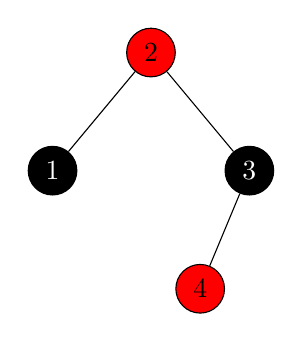
\begin{tikzpicture}[
                    red_node/.style={circle, draw=black, fill=red, minimum size=6mm},
                    black_node/.style={circle, draw=black, fill=black, text=white, minimum size=6mm},
                    level/.style={sibling distance=25mm/#1}
                ]
                    \node[red_node] {2}
                        child {
                            node[black_node] {1}
                        }
                        child {
                            node[black_node] {3}
                                child {
                                    node[red_node] {4}
                                }
                                child[missing] {}
                        };
                \end{tikzpicture}
                \caption{flatten T = [1,2,3,4]}
            \end{minipage}\hfill
            \begin{minipage}[t]{0.45\linewidth}
                \centering
                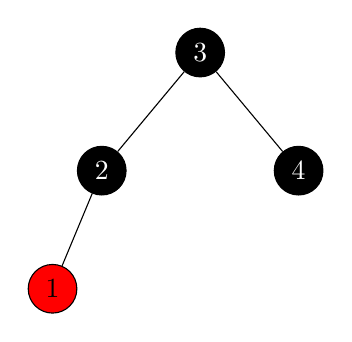
\begin{tikzpicture}[
                    red_node/.style={circle, draw=black, fill=red, minimum size=6mm},
                    black_node/.style={circle, draw=black, fill=black, text=white, minimum size=6mm},
                    level/.style={sibling distance=25mm/#1}
                ]
                    \node[black_node] {3}
                        child {
                            node[black_node] {2}
                                child {
                                    node[red_node] {1}
                                }
                                child[missing] {}
                        }
                        child {
                            node[black_node] {4}
                        };
                \end{tikzpicture}
                \caption{flatten T = [1,2,3,4]}
            \end{minipage}

            Use a quotient based on flatten.
        \end{figure}
    \end{frame}

    \begin{frame}{Properties of flatten}
        \begin{block}{Lemma(Extensionality)}
            $flatten (T1) = flatten (T2) \leftrightarrow \forall x, x \in T1 \leftrightarrow x \in T2$
        \end{block}
        \begin{block}{Proof}
            Idea:
                \begin{itemize}
                    \item two list are equal iff they are both sorted and permutations of each other
                    \item Ordered trees are sorted
                    \item Ordered trees are duplicate free: permutations
                \end{itemize}
        \end{block}
        \begin{block}{Lemma}
            size(T) = len(flatten(T))
        \end{block}
    \end{frame}

    \begin{frame}[fragile]{Don't do it twice}
        Mathlib data.set
        \begin{lstlisting}
        theorem mem_inter_iff (x : α) (a b : set α) :
            x ∈ a ∩ b ↔ (x ∈ a ∧ x ∈ b)
        \end{lstlisting}
        Kuratowski sets
        \begin{lstlisting}
        lemma in_intersection_iff_in_both {A:\text{{Type u}}} [decidable_eq A] (X Y: Kuratowski A) (a:A): kuratowski_member_prop a (X ∩ Y) = 
        (kuratowski_member_prop a X 
        ∧ kuratowski_member_prop a Y)
        \end{lstlisting}

    \end{frame}
    \begin{frame}{Finite by proof II}
        \begin{definition}
            A finite set $S_f$ is a pair of a set $S$ and a proof of its finiteness.
        \end{definition}
        \pause
        Examples
        \begin{enumerate}
            \item Bijection finite: $\exists (n:\mathbb{N}), (f: \mathbb{N} \to A).\; \text{{set.bij\_on}}\; f \;\{ x \in \mathbb{N} \mid x < n\} \;S$
            \item Surjection finite: $\exists (n:\mathbb{N}), (f: \mathbb{N} \to A).\; \text{{set.surj\_on}}\; f \;\{ x \in \mathbb{N} \mid x < n\} \;S $
            \item Dedekind finite: $\forall (S' \subsetneq S), (f: A \to A).\; \neg \text{{set.bij\_on}}\; f\; S'\; S$
        \end{enumerate}
    \end{frame}
    \begin{frame}[fragile]{Size}
        \begin{lstlisting}
        def is_finite {A: Type} (S: set A): Prop := 
            ∃ (n:ℕ) (f: ℕ → A), 
        set.bij_on f (set_of (λ (a:ℕ), a < n)) S

        noncomputable def size (s: set A) (fin: is_finite s): ℕ
         := classical.some fin
    \end{lstlisting}
    \end{frame}
\end{document}
